\documentclass{article}
\usepackage[screen]{geometry}
\usepackage{alltt,fancyvrb,framed,xcolor}
\usepackage[utf8]{inputenc}
\usepackage{listings,hyperref}
\usepackage{graphicx}
\colorlet{shadecolor}{yellow!30}   
\lstset{
    belowcaptionskip=1\baselineskip,
    xleftmargin=\parindent,
    breaklines=true, %% Wrap long lines
	language=C++,
	escapeinside={/*}{*/},
	escapebegin=\begin{shaded}\obeyspaces\obeylines,
	escapeend=\end{shaded},
    showstringspaces=false,
    basicstyle=\small\ttfamily,
    commentstyle=\itshape\color{gray},
    stringstyle=\color{black},
    keywordstyle=\bfseries\color{green},
    identifierstyle=\color{blue},
    %numbers=left,
}
\begin{document}
\tableofcontents

\newpage\section{Specification}
The program shows the fable of The Wolf and the
Kid through 4 scenes with one window of animation and another with the subtitles and sound.
If the user clicks on the animation, then the animation and sound pauses.
The animation starts off with a kid alone in a field with birds flying over him.
It then transitions into the wolf and kid walking towards each other accompanied.
Next, the Kid dances while the Wolf plays the pipe which can be heard.
Then, there is an abandoned field with an animated cloud where the Dog chases the wolf
into and soon jumps on the wolf allowing the Kid to escape.
Then, we learn the moral of the animation.

\newpage\section{Analysis}
\begin{description}
	\item [Input] There is a button that is used for user input. The button takes 
	place on the whole screen so the user will be able to click anywhere on the
	animation in order to pause and unpause the animation.
	\item [Process] There is a function called pauseCB that desribes that the 
	program automatically runs and when the user clicks on any part of the window,
	the movie will be paused. The pause is defined and called within the main.cpp 
	file within this lab in order for the function to work. The process of drawing
         parts of the characters and animating the birds will be 
         performed as individual functions are defined. There are 3 functions 
         defined to put together the total drawings of the wolf, goat, and dog. These
         3 functions work together in the drawCB2 file to put together the animation 
         of the movie on the second window. The first window shows the subtitles
         of what is going on in the instant of the animation. The first scene introduces
         the goat and shows the goat in the field all alone. In the second scene, we meet 
         the wolf who confronts the goat causing the goat to bargain for his life. In the 
         third scene, we see that the wolf and goat came to an agreement and the deal was
         that they would dance together while the wolf pipes a tune before the wolf's big 
         meal. The fourth scene shows that the dog heard the piping of the wolf and
         attacked the wolf so that the goat would be able to escape.
	\item [Output] If paused, the screen will be still until the user unpauses the animation.
	The output will be the animation of the 4 scenes of the fable
        with the subtitles showing up on a window next to the animation. The first scene 
         introduce the goat and shows the goat in the field all alone. In the second scene, we meet 
         the wolf who confronts the goat causing the goat to bargain for his life. In the 
         third scene, we see that the wolf and goat came to an agreement and the deal was
         that they would dance together while the wolf pipes a tune before the wolf's big 
         meal. The fourth scene shows that the dog heard the piping of the wolf and
         attacked the wolf so that the goat would be able to escape. The moral of the 
         story is “Do not let anything turn you from your purpose.”
	
\end{description}
\newpage\section{Design}

\begin{itemize}
	\item main.cpp was created as a main file
        to link all other functions into this and run
        together as an executable program. Then, the following
        functions were created.
        
	\item drawCB1.cpp This calls all of the functions in order for the first 
	window to successfully have the subtitles. The first thing
	to do is set the background to a clear color like gray
	and then make the font something legible and a size 
	big enough for anyone to read. Then, a file named 
	readFable was created so it is called upon in this function
	in order to read the fable that comes from the text file
	that the fable is written in. Each scene is split into a separate
	array so the time changes per scene would change the correct
	words on the subtitles window. The times for each scene are 
	defined in lab.h so that they only have to changed in one place
		
	\item drawCB2.cpp We start off the code with a few if statements
	that allow us to see that the backgrounds change
	according to what time it is. There are different
	backgrounds and that is seen by the different
	function names.Then, there is a scale command
	that will scale all of the vector characters that 
	have been created to be in this animation. 
	Once again, we manipulate if statements
	according to the timeline and when the time
	reaches a certain time, the scene will change into
	the next scene until the animation is over. Other 
	than using a translate function, there is a special
	function called pts[timeline] that uses gnuplot 
	data and points in order to create a Bezier curve
	in order to ensure that there is separate movement
	for all of the characters and so that all of the
	characters don't end up moving together.
	
	\item lab.h All information that needs to be repeated is put into file lab.h so 
	that an include statemnt can be used for the information rather than retyping
	 it several times in all of the different function files.
	 
	\item drawHead.cpp  This function is to draw the head of the wolf
         on the graphics window.

	\item drawEyes.cpp This function is to draw the eyes of the wolf
         on the graphics window.
         
	\item drawWolf.cpp  This function is to draw the wolf on the graphics window using
		the commands in it.

	\item mirrorY.cpp This function is to mirror the image on Y
         coordinate.
         
     \item scaler.cpp Scale is the unit size used for the x and y coordinates
		and that is set to what we need for the characters.
		
	\item moveCharacter.cpp This is the translate part of the animation and will cause the characters to move.
	
	\item drawBackground.cpp This gives the second window a background of a pasture so that the characters
	and birds are moving on top of the background rather than a blank screen.
	
	\item drawBackground1.cpp This gives the second window a background of the second scene so that the characters
are moving on top of the background rather than a blank screen. 
	
	\item drawBackground2.cpp This gives the second window a background of the third scene so that the characters
are moving on top of the background rather than a blank screen. 
	
	\item drawBackground3.cpp This gives the second window a background of the last scene so that the characters
and clouds are moving on top of the background rather than a blank screen. 
	
	\item drawBirds.cpp This is the animation of the birds moving around at the top of the window.
	
	\item getBirds.cpp This allows us to see the GIF of the birds run
	in the first scene through an if statement to see
	if there is outupt in the array to run the animation. 
	
	\item drawCloud.cpp This is the animation of the cloud moving around at the top of the window.
	
	\item drawBody.cpp The head of the wolf is drawn to the graphics window.
	
	\item drawdbody.cpp The body of the dog is drawn to the graphics window.
	
	\item drawdear1.cpp The left ear of the dog is drawn to the graphics window.
	\item drawdear2.cpp The right ear of the dog is drawn to the graphics window.
	
	\item drawdhead.cpp The dog's head is drawn to the graphics window.
	\item drawdleg1.cpp The dog's left leg is drawn to the graphics window.
	\item drawdleg2.cpp The dog's right leg is drawn to the graphics window.
	
	\item drawDog.cpp All of the functions to draw the dog are combined in this function to draw the total dog.
	
	\item drawGoat.cpp All of the functions to draw the goat are combined in this function to draw the total goat.
	\item drawLeg1.cpp  The wolf's left leg is drawn to the graphics window.
	\item draw Leg2.cpp The wolf's right leg is drawn to the graphics window.
	\item drawNose.cpp The wolf's nose is drawn to the graphics window.
	\item drawTail.cpp The wolf's tail is drawn to the graphics window.
	
	\item gBody.cpp The goat's body is drawn to the graphics window.
	\item gEye.cpp The goat's eye is drawn to the graphics window.
	\item gHead.cpp The goat's head is drawn to the graphics window.
	\item gHorn1.cpp The goat's left horn is drawn to the graphics window.
	\item gHorn2.cpp The goat's right horn is drawn to the graphics window.
	\item gLeg1.cpp The goat's right leg is drawn to the graphics window.
	\item gLeg2.cpp The goat's left leg is drawn to the graphics window.
	\item gTail.cpp The goat's tail is drawn to the graphics window.
	\item fables.txt Our team fable is called from here rather than
	individually typing it out.
	\item readFable.cpp Our fable is read from a file rather than written
	directly on the screen.
	\item showText.cpp The text of our fable is shown on a screen that is 
	right next to that of the animation and which is time synced. 
	\item getPoints.cpp This function gets points from the data files 
	that was written in gnuplot and the points
	would follow the bezier curve and so it is called
	here in order for each character to have its
	own path.
	\item getPoints2.cpp This function gets points2 from the data2 files 
	that was written in gnuplot and the points2
	would follow the bezier curve and so it is called
	here in order for each character to have its
	own path.
	\item getPoints3.cpp This function gets points3 from the data3 files 
	that was written in gnuplot and the points3
	would follow the bezier curve and so it is called
	here in order for each character to have its
	own path.
	\item soundEffects.cpp This allows the animation to have 
	sound to enhance what the characters are 
	doing. The sounds play along with the
	timeline and approximately when the
	scenes change to represent what is going on.
	The sound bits were uploaded to our 
	directory in order for it to work.
	
         
         
\end{itemize}
\newpage\section{Implementation}
\subsection{main.cpp}\lstinputlisting{main.cpp}
\newpage\subsection{drawCB1.cpp}\lstinputlisting{drawCB1.cpp}
\newpage\subsection{drawCB2.cpp}\lstinputlisting{drawCB2.cpp}
\newpage\subsection{lab.h}\lstinputlisting{lab.h}
\newpage\subsection{drawhead.cpp}\lstinputlisting{drawHead.cpp}
\newpage\subsection{drawEyes.cpp}\lstinputlisting{drawEyes.cpp}
\newpage\subsection{drawWolf.cpp}\lstinputlisting{drawWolf.cpp}
\newpage\subsection{mirrorY.cpp}\lstinputlisting{mirrorY.cpp}
\newpage\subsection{scaler.cpp}\lstinputlisting{scaler.cpp}
\newpage\subsection{moveCharacter.cpp}\lstinputlisting{moveCharacter.cpp}
\newpage\subsection{drawBackground.cpp}\lstinputlisting{drawBackground.cpp}
\newpage\subsection{drawBackground1.cpp}\lstinputlisting{drawBackground1.cpp}
\newpage\subsection{drawBackground2.cpp}\lstinputlisting{drawBackground2.cpp}
\newpage\subsection{drawBackground3.cpp}\lstinputlisting{drawBackground3.cpp}
\newpage\subsection{drawBirds.cpp}\lstinputlisting{drawBirds.cpp}
\newpage\subsection{getBirds.cpp}\lstinputlisting{getBirds.cpp}
\newpage\subsection{drawCloud.cpp}\lstinputlisting{drawCloud.cpp}
\newpage\subsection{drawBody.cpp}\lstinputlisting{drawBody.cpp}
\newpage\subsection{drawdbody.cpp}\lstinputlisting{drawdbody.cpp}
\newpage\subsection{drawdear1.cpp}\lstinputlisting{drawdear1.cpp}
\newpage\subsection{drawdear2.cpp}\lstinputlisting{drawdear2.cpp}
\newpage\subsection{drawdhead.cpp}\lstinputlisting{drawdhead.cpp}
\newpage\subsection{drawdleg1.cpp}\lstinputlisting{drawdleg1.cpp}
\newpage\subsection{drawdleg2.cpp}\lstinputlisting{drawdleg2.cpp}
\newpage\subsection{drawDog.cpp}\lstinputlisting{drawDog.cpp}
\newpage\subsection{drawGoat.cpp}\lstinputlisting{drawGoat.cpp}
\newpage\subsection{drawLeg1.cpp}\lstinputlisting{drawLeg1.cpp}
\newpage\subsection{drawLeg2.cpp}\lstinputlisting{drawLeg2.cpp}
\newpage\subsection{drawNose.cpp}\lstinputlisting{drawNose.cpp}
\newpage\subsection{drawTail.cpp}\lstinputlisting{drawTail.cpp}
\newpage\subsection{gBody.cpp}\lstinputlisting{gBody.cpp}
\newpage\subsection{gEye.cpp}\lstinputlisting{gEye.cpp}
\newpage\subsection{gHead.cpp}\lstinputlisting{gHead.cpp}
\newpage\subsection{gHorn1.cpp}\lstinputlisting{gHorn1.cpp}
\newpage\subsection{gHorn2.cpp}\lstinputlisting{gHorn2.cpp}
\newpage\subsection{gLeg1.cpp}\lstinputlisting{gLeg1.cpp}
\newpage\subsection{gLeg2.cpp}\lstinputlisting{gLeg2.cpp}
\newpage\subsection{gTail.cpp}\lstinputlisting{gTail.cpp}
\newpage\subsection{fables.txt}\lstinputlisting{fables.txt}
\newpage\subsection{readFable.cpp}\lstinputlisting{readFable.cpp}
\newpage\subsection{showText.cpp}\lstinputlisting{showText.cpp}
\newpage\subsection{getPoints.cpp}\lstinputlisting{getPoints.cpp}
\newpage\subsection{getPoints2.cpp}\lstinputlisting{getPoints2.cpp}
\newpage\subsection{getPoints3.cpp}\lstinputlisting{getPoints3.cpp}
\newpage\subsection{soundEffects.cpp}\lstinputlisting{soundEffects.cpp}
\section{Test}
\subsection{Testcase 1}
\includegraphics[scale=0.5]{Scene1.png}
\newline This shows Scene 1.
\newpage\subsection{Testcase 2}
\includegraphics[scale=0.5]{Scene2.png}
\newline This shows Scene 2.
\newpage\subsection{Testcase 3}
\includegraphics[scale=0.5]{Scene3.png}
\newline This shows Scene 3.
\newpage\subsection{Testcase 4}
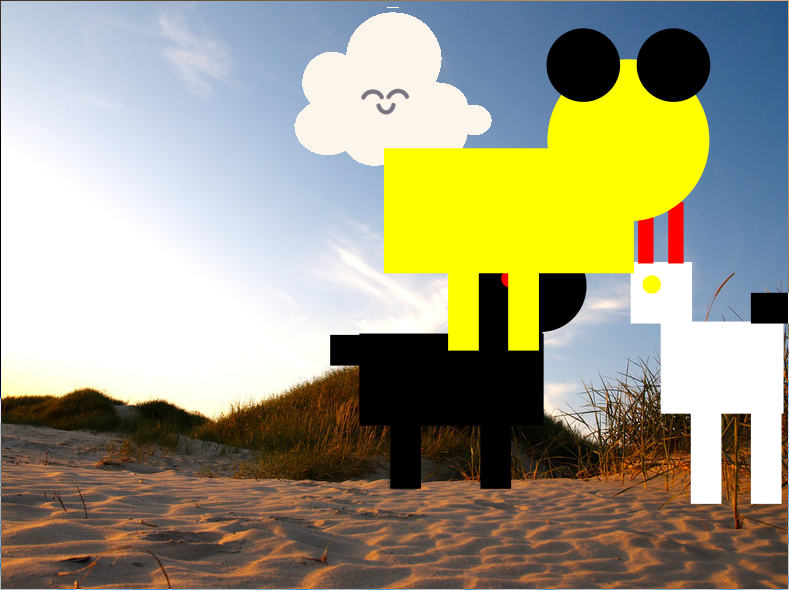
\includegraphics[scale=0.5]{Scene4.png}
\newline This shows Scene 4.
\newpage\subsection{Test cont.} 
The program meets the requreiments with the expected output and the images taken 
of program running showing the actual results.
\end{document}
